\section{Implementación}\label{sec:implementacion}
\begin{frame}{Diagrama UML}
\begin{center}
    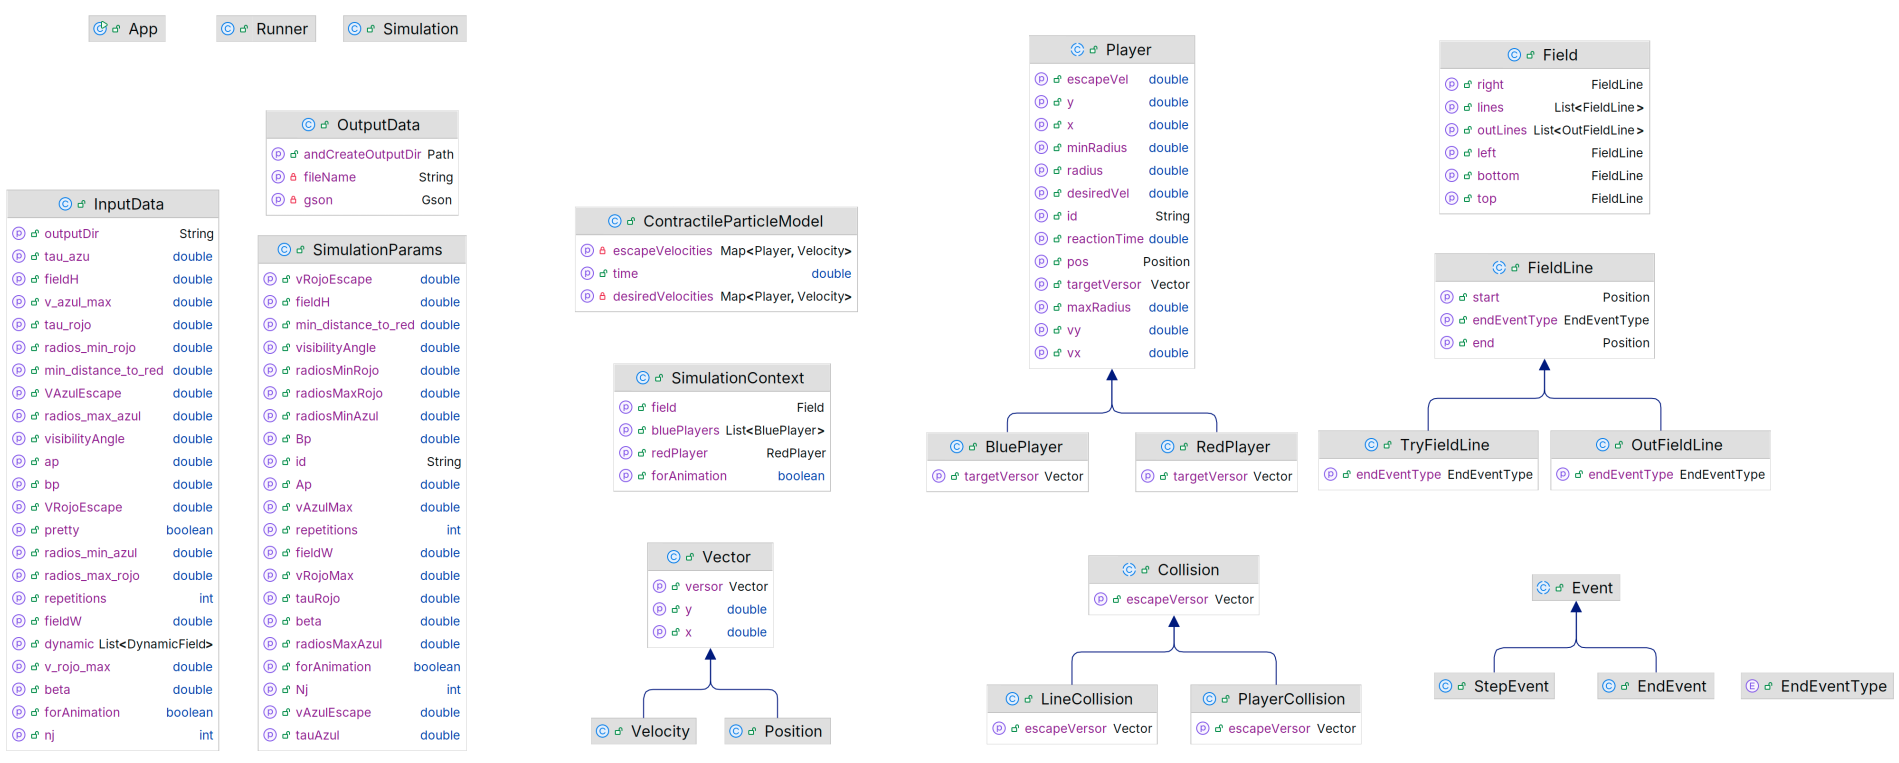
\includegraphics[width=\textwidth]{pic/03-implementacion/UML}
\end{center}
\end{frame}

\begin{frame}{Pseudocódigo}
    \tiny{
        \begin{algorithmic}
            \State \textbf{Simulación:}
            \State \text{Generar: campo, jugadores azules (uniformemente distribuidos) y jugador rojo}
            \While{\text{true}}
                \For{\text{cada jugador}}
                    \State \text{Preguntar su dirección objetivo deseada segun heuristica}
                    \State \text{Calcular el vector velocidad en función del modelo operativo y direccón objetivo}
                \EndFor
                \State \text{Pasar dt tiempo}
                \For{\text{cada jugador}}
                    \State \text{Actualizar posición}
                \EndFor
                \If{\text{jugador rojo está sobre linea izquierda}}
                    \State \text{Emitir evento $try$}
                    \State \text{break}
                \ElsIf{\text{jugador rojo está sobre cualquier otra linea}}
                    \State \text{Emitir evento $out$}
                    \State \text{break}
                \ElsIf{\text{algún jugador azul se solapa con el rojo}}
                    \State \text{Emitir evento $tackle$}
                    \State \text{break}
                \EndIf
            \EndWhile
        \end{algorithmic}
    }
\end{frame}
